\chapter{Methoden und Materialien}

\section{Software/Programme}

Für die RAGs und die Bewertung der RAGs werden Tools benötigt. Im Nachfolgenden werden diese Tools genauer erklärt.

\subsection{Ollama}
Ollama~\cite{ollama_2025} ist ein Open-Source LLM-Server, der auf einem eigenen Computer oder in der Cloud ausgeführt wird.
Es können verschiedene Open-Source LLMs und Embedding-Modelle ausgeführt werden. In der vorliegenden Arbeit werden die Modelle ollama/nomic-embed-text und ollama/deepseek-r1:32b verwendet. 

\subsection{Embeddings}
Vektoren sind die Beschreibung einer Position im mehrdimensionalen Raum. Es handelt sich hier meist um Positionen, welche mehrere tausend Dimensionen haben.
Embeddings ermöglichen die Darstellung von z. B. Wörtern im mehrdimensionalen Raum.
Je näher zwei Wörter im Raum beieinander sind, desto ähnlicher sind sie.
Welche Embeddings für welche Versuche genutzt werden, wird in Kapitel~\ref{sec:bewertung} \enquote{Bewertung} beschrieben.

\subsection{Vektordatenbank ChromaDB}
ChromaDB~\cite{trychroma_2025} ist eine Open-Source-Vektordatenbank, die zur persistenten Speicherung und effizienten Abfrage von hochdimensionalen Embeddings eingesetzt wird.
Die Vektordatenbank ist also ein fester Bestandteil des RAGs und wird sowohl für die Open-Source-Modelle als auch für die Closed-Source-Modelle von z.B. OpenAI benutzt. Dies schafft eine einheitlichere Basis zum Vergleichen der LLMs.

\subsection{RAGAS}
RAGAS ist ein Open-Source-Tool und liefert neben dem Tool selbst hilfreiche Dokumentation für die Metriken und die Bewertung von RAGs~\cite{es-etal-2024-ragas}.
Es werden Funktionen wie die automatische Generierung von Interessengruppen, die Testset-Generierung und die Bewertung von RAGs anhand von Testsets bereitgestellt.
Für diese Arbeit sind die Funktionen der Testset-Generierung und die damit ermöglichte Bewertung der RAGs relevant.

Was RAGAS von Giskard und Comet unterscheidet, ist, dass keine \glqq reference answer\grqq{} benötigt wird.
RAGAS ist mit 9400 Sternen bei Github beliebt, dazu trägt sicherlich auch die gute Integration mit vielen anderen Werkzeugen bei.

\subsection{Langchain}
Langchain~\cite{langchain_framework} ist ein Framework, das bei der Entwicklung von Anwendungen, die LLMs nutzen, eine erhebliche Hilfe ist.
Durch die vielen Komponenten und Integrationen wichtiger Tools bietet es die Grundlage für die Verbindung von Daten und komplexen Workflows.
In dieser Arbeit wird Langchain genutzt, um die Vektordatenbank und Ollama mit RAGAS zu verbinden. Genutzt wurde die Version 0.3.25.

\section{Daten}
Da in dieser Arbeit die Nutzung von RAG-Evaluation-Tools für betriebliche Abläufe untersucht werden soll, werden zum Teil echte, nicht generierte Dokumente – im Folgenden \enquote{Originaldokumente} genannt – verwendet.
Da die Menge an Originaldokumenten begrenzt ist, werden diese mit synthetischen Daten ergänzt.

\subsection{Originaldokumente}
Die Dokumente stammen aus Unterlagen des Einzelunternehmens \enquote{Develop 4 Future (D4F)}, das vereinfachte CMS-Webseiten für Grundschulen entwickelt hat.
Der Einzelunternehmer hinter D4F war der Autor.
Die Unternehmung wird nicht mehr aktiv verfolgt und die anonymisierten Daten können ohne Bedenken für diese Arbeit genutzt werden.
In den Versuchen wurden drei unterschiedliche Anzahlen an Dokumenten getestet: 10, 100 und 400.
Aus den Unterlagen von D4F ließen sich 73 nutzbare Originaldokumente finden.
Neben den Originaldokumente, welche Businesspläne, Finanzpläne, aber auch Elternbriefe umfassen, gibt es den dazugehörigen Code, der für die Programmierung von Webseiten verwendet wurde.
Dieser besteht aus drei Projekten:
\begin{enumerate}
    \item Die Webseite, die öffentlich zugänglich ist
    \item dem Admin-Bereich, welcher nur für das Personal der Grundschule zugänglich ist
    \item dem Backend, welches die Daten verwaltet.
\end{enumerate}
Für die Versuche mit zehn Dokumenten wurden nur \enquote{Originaldokumente} genutzt.

\subsubsection{Originaldokument Beispiel}
Ein typisches Origianldokument sieht wie folgt aus:

\textbf{Anfang: \enquote{SmartKlassenzimmer\_Risikoanalyse.txt}}
\begin{quote}
Risikoanalyse für das Projekt \enquote{SmartKlassenzimmer}

Risiko: Verzögerungen bei der Hardware-Lieferung\\
Maßnahme: Verträge mit mehreren Lieferanten, Pufferzeiten im Zeitplan

Risiko: Technische Probleme bei der Installation\\
Maßnahme: Vorab-Tests, erfahrenes Technik-Team, Notfallplan

Risiko: Akzeptanzprobleme bei Lehrkräften\\
Maßnahme: Umfassende Schulungen, Einbindung in die Entwicklung

Risiko: Datenschutzverletzungen\\
Maßnahme: Strenge Zugriffskontrollen, regelmäßige Audits, DSGVO-konforme Prozesse

Risiko: Budgetüberschreitung\\
Maßnahme: Monatliche Kostenkontrolle, Reserven im Budget

Risiko: Geringe Nutzung der Plattform durch Schüler:innen\\
Maßnahme: Motivierende Inhalte, Feedbackrunden, Anpassung der Funktionen
\end{quote}
\textbf{Ende}


\subsection{Synthetische Daten}
Um von 73 gegebenen Dokumenten auf 100 Dokumente zu kommen, wurden mithilfe von LLMs synthetisch weitere Dokumente generiert.
Beim Generieren der Dokumente wurden dem LLM die bisherigen Dokumente zur Verfügung gestellt und komplett neue Bereiche/Projekte erfunden. Diese bestehen dann aus Kostenplanungen, Zeitplänen und Elternbriefen für Datenschutzinformationen.

\subsection{Anwendungsszenarien}
Die folgenden drei Stufen wurden gewählt, um typische Anwendungsszenarien realistisch abzubilden:
\begin{enumerate}
    \item \textbf{10 Dokumente:} Ein einzelner Anwendungsfall – das RAG-System wird nur temporär genutzt und danach verworfen.
    \item \textbf{100 Dokumente:} Kontinuierliche Nutzung durch eine Einzelperson – das System wächst schrittweise über die Zeit hinweg.
    \item \textbf{400 Dokumente:} Gemeinsame Nutzung durch mehrere Personen – das RAG muss verschiedene Themenbereiche abdecken und eine breitere Wissensbasis verwalten.
\end{enumerate}

\section{Fragebögen}

Die Generierung von Fragebögen ist eines der Alleinstellungsmerkmale von RAGAS.
Sie sind die Grundlage für die Bewertung der RAGs. Es gibt unterschiedliche Fragetypen, die unterschiedliche Aspekte der RAG-Performance evaluieren.

\subsection{Fragetypen}

RAGAS unterstützt verschiedene Fragetypen für die Testset-Generierung, die unterschiedliche Aspekte der RAG-Performance evaluieren.
Abbildung~\ref{fig:ragas_query_types} zeigt die verschiedenen Fragetypen, die RAGAS für die Evaluation von RAG-Systemen verwendet:

\begin{figure}[h!]
    \centering
    \begin{tikzpicture}[
        node distance=1cm and -0.5cm,
        every node/.style={draw=orange, fill=white, rounded corners, minimum width=3.2cm, minimum height=1cm, align=center},
        arrow/.style={-{Latex}, thick}
    ]

        % Top-level node
        \node (queries) {Queries};

        % Second level
        \node (singlehop) [below left=of queries] {Single-Hop Query};
        \node (multihop)  [below right=of queries] {Multi-Hop Query};

        % Third level - Single-Hop children
        \node (sh-specific) [below left=of singlehop, xshift=0cm] {Specific Query};
        \node (sh-abstract) [below right=of singlehop, xshift=-2cm] {Abstract Query};

        % Third level - Multi-Hop children
        \node (mh-specific) [below left=of multihop, xshift=2cm] {Specific Query};
        \node (mh-abstract) [below right=of multihop, xshift=0cm] {Abstract Query};

        % Edges
        \draw[arrow] (queries) -- (singlehop);
        \draw[arrow] (queries) -- (multihop);

        \draw[arrow] (singlehop) -- (sh-specific);
        \draw[arrow] (singlehop) -- (sh-abstract);

        \draw[arrow] (multihop) -- (mh-specific);
        \draw[arrow] (multihop) -- (mh-abstract);

    \end{tikzpicture}
    \caption[Fragetypen in RAGAS]{Fragetypen in RAGAS \cite{ragas_test_data_generation}}
    \label{fig:ragas_query_types}
\end{figure}


Diese in Abbildung~\ref{fig:ragas_query_types} gezeigten verschiedenen Fragetypen ermöglichen es, unterschiedliche Aspekte der RAG-Performance zu testen.
Während spezifische Fragen häufig mit einer einzigen Anfrage an die Wissensdatenbank beantwortet werden können, benötigen abstrakte Fragen eine Erklärung.
In der RAGAS-Dokumentation \cite{ragas_query_types} wird für konkrete Fragen das Beispiel gegeben: \enquote{Wann hat Einstein die Relativitätstheorie veröffentlicht?}.
Eine abstraktere Frage wäre: \glqq Wie hat Einsteins Relativitätstheorie unser Verständnis der Welt verändert?\grqq{}

Bei Multi-Hop-Queries handelt es sich um Fragen, die mehr als eine Wissensabfrage benötigen. Die Frage \glqq Welche Wissenschaftler haben Einsteins Relativitätstheorie beeinflusst und welche Theorie haben sie vorgeschlagen?\grqq{} benötigt erst eine Abfrage, um die Wissenschaftler herauszufinden, und dann weitere, um die jeweils vorgeschlagene Theorie abzufragen.
Für die abstrakte Multi-Hop-Query kann man wieder nach einer Erklärung für den Inhalt und wie sich dieser über die Zeit verändert hat, fragen.

Diese Unterscheidung wird getroffen, um sowohl sehr gezielte Wissensabfragen als auch abstraktere Abfragen über mehrere Dokumente zu testen.

\subsection{Wissensgraph}

Für die eben erwähnten Multi-Hop-Queries müssen aus den gegebenen Dokumenten Themen, die zusammenhängen, aber nicht direkt im gleichen Dokument vorkommen, gefunden werden.
Da dies bei großen Datensätzen manuell oder selbst mit einem LLM schwierig ist, wird ein Wissensgraph erstellt. \\
Dies geschieht in drei Schritten. Zuerst werden die Dokumente beim sogenannten Chunking in kleinere Einheiten (Knoten) unterteilt.
Aus diesen Einheiten können dann Entitäten wie z.B. Namen (Einstein) oder Schlüsselbegriffe (Relativitätstheorie) extrahiert werden.
Im letzten Schritt werden dann Verbindungen zwischen Knoten hergestellt, dies wird in der Abbildung~\ref{fig:chunk-beziehungen} dargestellt.

\begin{figure}[h!]
    \centering
    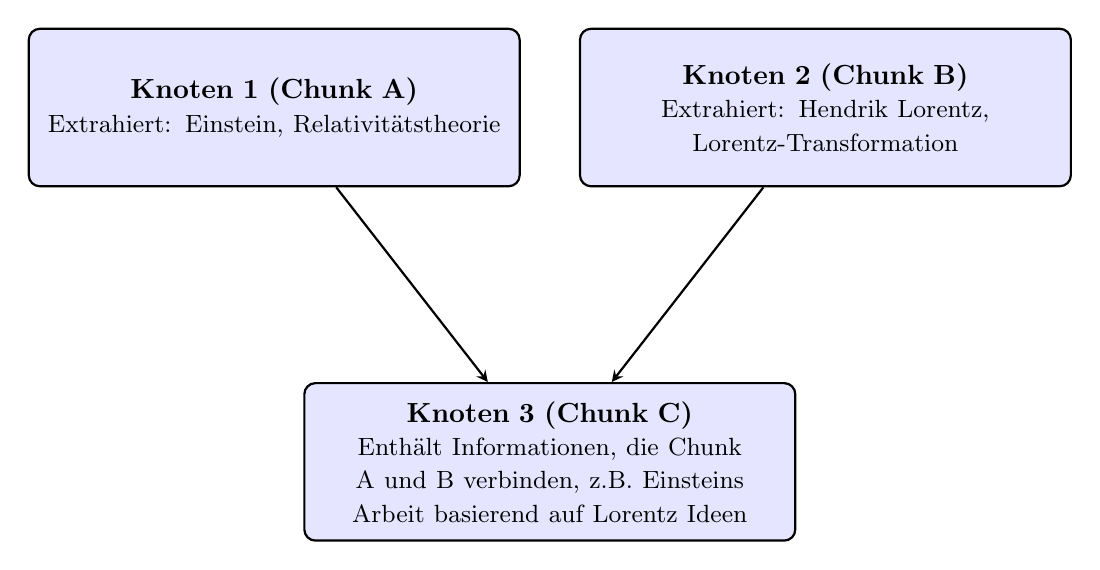
\begin{tikzpicture}[node distance=10cm, auto,>=stealth, thick,
    % Stile für die Knoten (repräsentieren Dokumenten-Chunks)
        chunk/.style={rectangle, rounded corners, draw=black, fill=blue!10, text width=6cm, text centered, minimum height=2cm},
    % Stil für die Kanten (repräsentieren Beziehungen)
        relation/.style={->, draw=black}]

        % Knoten für die Dokumenten-Chunks definieren
        \node[chunk] (n1) at (0,0) {\textbf{Knoten 1 (Chunk A)}\\ \small Extrahiert: Einstein, Relativitätstheorie};
        \node[chunk] (n2) at (7,0) {\textbf{Knoten 2 (Chunk B)}\\ \small Extrahiert: Hendrik Lorentz, Lorentz-Transformation};
        \node[chunk] (n3) at (3.5,-4.5) {\textbf{Knoten 3 (Chunk C)}\\ \small Enthält Informationen, die Chunk A und B verbinden, z.B. Einsteins Arbeit basierend auf Lorentz Ideen};

        % Kanten zeichnen, die Beziehungen zwischen den Chunks darstellen
        \draw[relation] (n1) -- (n3);
        \draw[relation] (n2) -- (n3);
    \end{tikzpicture}
    \caption[Beziehungen zwischen Dokumenten-Chunks]{Beziehungen zwischen Dokumenten-Chunks: Chunk C verbindet die Inhalte von Chunk A und B.}
    \label{fig:chunk-beziehungen}
\end{figure}

Für die Daten aus den Versuchen mit 100 Dokumenten hat RAGAS 27 Themen identifiziert. Unter anderem wurden folgende Themen gefunden:
Finanzmanagement, Bildungsprojekt Digitalisierung, Projektmanagement und Planung, Zuwendungsverwaltung, Break-Even-Analyse, Finanzplanung und Investitionen, Finanzplanung und Liquidität.